\documentclass{beamer}

\mode<presentation>
{
  \usetheme{default}
  \usecolortheme{default}
  \usefonttheme{default}
  \setbeamertemplate{navigation symbols}{}
  \setbeamertemplate{caption}[numbered]
  \setbeamertemplate{footline}[page number]
  \setbeamercolor{frametitle}{fg=white}
  \setbeamercolor{footline}{fg=black}
} 

\usepackage[english]{babel}
\usepackage[utf8x]{inputenc}
\usepackage{tikz}
\usepackage{listings}
\usepackage{courier}
\usepackage{array}
\usepackage{bold-extra}
\usepackage{minted}

\xdefinecolor{darkblue}{rgb}{0.1,0.1,0.7}
\xdefinecolor{darkgreen}{rgb}{0,0.5,0}
\xdefinecolor{darkgrey}{rgb}{0.35,0.35,0.35}
\xdefinecolor{darkorange}{rgb}{0.8,0.5,0}
\xdefinecolor{darkred}{rgb}{0.7,0,0}
\xdefinecolor{dianablue}{rgb}{0.18,0.24,0.31}
\definecolor{commentgreen}{rgb}{0,0.6,0}
\definecolor{stringmauve}{rgb}{0.58,0,0.82}

\lstset{ %
  backgroundcolor=\color{white},      % choose the background color
  basicstyle=\ttfamily\small,         % size of fonts used for the code
  breaklines=true,                    % automatic line breaking only at whitespace
  captionpos=b,                       % sets the caption-position to bottom
  commentstyle=\color{commentgreen},  % comment style
  escapeinside={\%*}{*)},             % if you want to add LaTeX within your code
  keywordstyle=\color{blue},          % keyword style
  stringstyle=\color{stringmauve},    % string literal style
  showstringspaces=false,
  showlines=true
}

\lstdefinelanguage{scala}{
  morekeywords={abstract,case,catch,class,def,%
    do,else,extends,false,final,finally,%
    for,if,implicit,import,match,mixin,%
    new,null,object,override,package,%
    private,protected,requires,return,sealed,%
    super,this,throw,trait,true,try,%
    type,val,var,while,with,yield},
  otherkeywords={=>,<-,<\%,<:,>:,\#,@},
  sensitive=true,
  morecomment=[l]{//},
  morecomment=[n]{/*}{*/},
  morestring=[b]",
  morestring=[b]',
  morestring=[b]"""
}

\title[2017-05-23-ecosystem-femtocode]{Femtocode: querying HEP data}
\author{Jim Pivarski}
\institute{Princeton University -- DIANA}
\date{May 23, 2017}

\begin{document}

\logo{\pgfputat{\pgfxy(0.11, 8)}{\pgfbox[right,base]{\tikz{\filldraw[fill=dianablue, draw=none] (0 cm, 0 cm) rectangle (50 cm, 1 cm);}}}\pgfputat{\pgfxy(0.11, -0.6)}{\pgfbox[right,base]{\tikz{\filldraw[fill=dianablue, draw=none] (0 cm, 0 cm) rectangle (50 cm, 1 cm);}\includegraphics[height=0.99 cm]{diana-hep-logo.png}\tikz{\filldraw[fill=dianablue, draw=none] (0 cm, 0 cm) rectangle (4.9 cm, 1 cm);}}}}

\begin{frame}
  \titlepage
\end{frame}

\logo{\pgfputat{\pgfxy(0.11, 8)}{\pgfbox[right,base]{\tikz{\filldraw[fill=dianablue, draw=none] (0 cm, 0 cm) rectangle (50 cm, 1 cm);}\includegraphics[height=1 cm]{diana-hep-logo.png}}}}

% Uncomment these lines for an automatically generated outline.
%\begin{frame}{Outline}
%  \tableofcontents
%\end{frame}

%%%%%%%%%%%%%%%%%%%%%%%%%%%%%%%%%%%%%%%%%%%%%%%%%%%%%%%

\begin{frame}{A data analyst's life}
\vspace{0.5 cm}
\hfill Reducing a large set of files

\hfill into a small set of files

\hfill to make plots.

\vspace{-1.5 cm}
\includegraphics[width=\linewidth]{stack-of-files.png}

\vspace{0.5 cm}
The last dataset must be small enough to permit \textcolor{darkblue}{\underline{real time}} plotting and re-plotting.
\end{frame}

\begin{frame}{This is a problem}
\begin{center}
\begin{minipage}{0.8\linewidth}
\Large
\textcolor{darkblue}{Assertion:} if physicists {\it could} make plots \textcolor{gray}{(and other aggregations for statistical analysis)} directly from the collaboration's Analysis Object Data in real time, they {\it would.}
\end{minipage}
\end{center}
\end{frame}

\begin{frame}{Database-style interaction}
\vspace{0.5 cm}
\textcolor{darkblue}{Rapid queries on big data are possible; in fact, it's a big field:}

\vspace{0.5 cm}
\mbox{\hspace{-1 cm}
\includegraphics[height=1.23 cm]{sparksql-logo.png}
\includegraphics[height=1.23 cm]{impala-logo.png}
\includegraphics[height=1.23 cm]{ibis-logo.png}
\includegraphics[height=1.23 cm]{kudu-logo.png}
\includegraphics[height=1.23 cm]{hawk-logo.png}
\includegraphics[height=1.23 cm]{drill-logo.png}
\includegraphics[height=1.23 cm]{dremel-logo.png}
\includegraphics[height=1.23 cm]{bigquery-logo.png}}

\vspace{0.5 cm}
\begin{itemize}\setlength{\itemsep}{0.25 cm}
\item<2-> Instead of users maintaining private skims, running local processes, they \textcolor{darkblue}{\underline{share}} a distributed query server.
\item<3-> Instead of fetching data from disk, \textcolor{darkblue}{\underline{cache}} \mbox{in RAM/SSD/X-Point.\hspace{-1 cm}}
\item<4-> Instead of evaluating user's code as-is, \textcolor{darkblue}{\underline{translate}} it into a form that optimizes memory bandwidth.
\item<5-> Instead of executing operations on objects, execute on \textcolor{darkblue}{\underline{flat arrays}} of (columns) numbers.
\end{itemize}
\end{frame}

\begin{frame}{\underline{Sharing} and \underline{caching} go together}
\vspace{0.25 cm}
Most users need mostly the same input variables.
\begin{itemize}
\item For instance, all muon analyses use the same kinematic variables and may use different isolation variables.
\item Exact fraction is unknown, but we know that analysis groups share ntuplizers that slim the same 10\% (4~kB/event) of CMS MiniAOD.
\end{itemize}

%% \vspace{0.5 cm}
%% \begin{columns}[t]
%% \column{0.5\linewidth}
%% \textcolor{darkblue}{Case 1:}

%% \textcolor{darkblue}{\underline{Users share a remote database}}

%% \vspace{0.1 cm}
%% Shared inputs are in cache once.

%% \vspace{2\baselineskip}
%% \vspace{0.1 cm}
%% Unique requirements separately cached.

%% \column{0.5\linewidth}
%% \textcolor{darkblue}{Case 2:}

%% \textcolor{darkblue}{\underline{Divide resources among users}}

%% \vspace{0.1 cm}
%% Shared inputs are separately in cache in each user's process (duplicated in different places).

%% \vspace{0.1 cm}
%% Unique requirements separately cached (same).
%% \end{columns}

\vspace{0.5 cm}
If, say, half of the variables are shared and half are not, a server distributed across a cluster with 10~TB of RAM \textcolor{darkblue}{effectively gives each user 5~TB~$+$~$\epsilon$ of RAM.}
\end{frame}

\begin{frame}{\underline{Sharing} and \underline{columnar} data go together}
\vspace{0.5 cm}
Columns for a dataset do not need to come from the same file.

\begin{center}
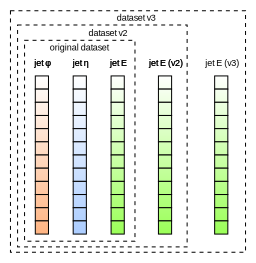
\includegraphics[width=0.6\linewidth]{virtual-datasets.pdf}
\end{center}

\vspace{-0.25 cm}
Extreme version of the ``friend TTree'' concept (superfriends).
\end{frame}

\begin{frame}{The limitation}
\mbox{\only<1>{\hspace{-0.75 cm}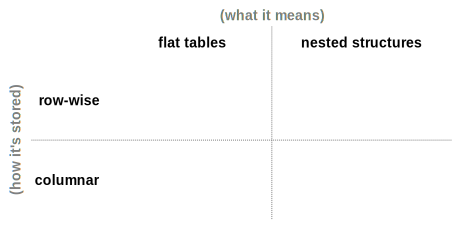
\includegraphics[width=1.15\linewidth]{table-of-formats.pdf}}\only<2>{\hspace{-0.75 cm}\includegraphics[width=1.15\linewidth]{table-of-formats2.pdf}}\only<3>{\hspace{-0.75 cm}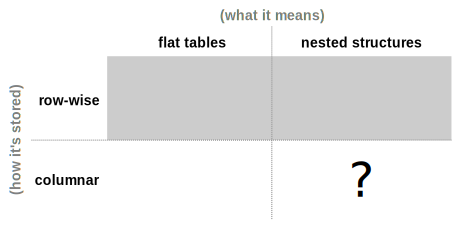
\includegraphics[width=1.15\linewidth]{table-of-formats3.pdf}}}
\end{frame}

\begin{frame}[fragile]{Femtocode: query language and engine}
\vspace{0.5 cm}
\begin{columns}[t]
\column{0.5\linewidth}
\textcolor{darkblue}{\Large \underline{Physicist's view}}

\small
\vspace{0.25 cm}
{\bf Muon object schema:}

\scriptsize
\vspace{-0.1 cm}
\begin{verbatim}
collection(record(
    pt = real(0, almost(inf)),
    eta = real,
    phi = real(-pi, pi)))
\end{verbatim}

\small
\vspace{0.25 cm}
{\bf Example query:}

\scriptsize
\begin{minted}{scala}
muons.filter(mu => mu.pt > 5)
     .map(mu => mu.pt*sinh(mu.eta))
     .max
\end{minted}

\small
\vspace{0.25 cm}
{\bf Return type:}

\scriptsize
\vspace{-0.1 cm}
\begin{verbatim}
union(null, real)
\end{verbatim}

\column{0.55\linewidth}
\textcolor{darkblue}{\Large \underline{Execution engine}}

\small
\vspace{0.25 cm}
{\bf Physical representation:}

\scriptsize
\vspace{-0.1 cm}
\begin{verbatim}
muons.pt:   [31.09, 9.76, 8.18, ...]
muons.phi:  [-0.48, 0.12, 0.12, ...]
muons.eta:  [0.88, 0.92, -0.26, ...]
muons@size: [3, 1, 1, 2, ...]
\end{verbatim}

\small
\vspace{0.25 cm}
{\bf Example execution:}

\scriptsize
\begin{enumerate}
\item Compute {\tt\scriptsize muons.pt > 5} for {\it all} muons.
\item Compute {\tt\scriptsize sinh(muons.eta)} for elements in which {\tt\scriptsize \#1} is true.
\item Compute {\tt\scriptsize muons.pt * \#2} for elements in which {\tt\scriptsize \#1} is true.
\item Pick the maximum {\tt\scriptsize \#3} value or {\tt\scriptsize NaN}, returning array with one value per event.
\end{enumerate}

\end{columns}
\end{frame}



\end{document}
